%%%%%%%%%%%%%%%%%%%%%%%%%%%%%%%%%%%%%%%%%
% Medium Length Professional CV
% LaTeX Template
% Version 3.0 (December 17, 2022)
%
% This template originates from:
% https://www.LaTeXTemplates.com
%
% Author:
% Vel (vel@latextemplates.com)
%
% Original author:
% Trey Hunner (http://www.treyhunner.com/)
%
% License:
% CC BY-NC-SA 4.0 (https://creativecommons.org/licenses/by-nc-sa/4.0/)
%
%%%%%%%%%%%%%%%%%%%%%%%%%%%%%%%%%%%%%%%%%

%----------------------------------------------------------------------------------------
%	PACKAGES AND OTHER DOCUMENT CONFIGURATIONS
%----------------------------------------------------------------------------------------

\PassOptionsToPackage{dvipdfmx}{graphicx}
\documentclass[
	%a4paper, % Uncomment for A4 paper size (default is US letter)
	11pt, % Default font size, can use 10pt, 11pt or 12pt
]{resume} % Use the resume class

\usepackage{libertine} % English: Linux Libertine (same as the thesis)
\usepackage{libertinust1math}
\usepackage[haranoaji]{pxchfon} % Japanese: Harano Aji Mincho / Gothic (same as the thesis)
\usepackage[dvipdfmx,linkcolor=blue,anchorcolor=blue,urlcolor=blue,colorlinks=true]{hyperref}
\urlstyle{same}
\usepackage{pxjahyper}
\usepackage{needspace}
\usepackage{xurl} % URLを任意の場所で折り返せるようにする
\usepackage[dvipdfmx,linkcolor=blue,anchorcolor=blue,urlcolor=blue,colorlinks=true]{hyperref}
% 写真について
\usepackage[absolute,overlay]{textpos}
\usepackage{graphicx} % dvipdfmx は文書クラスより前の \PassOptionsToPackage で指定

\setlength{\TPHorizModule}{1mm}
\setlength{\TPVertModule}{1mm}


\name{日下部 完 {\small（くさかべ かん）}}
\address{1999年8月6日生（26歳） / 性別：男}
% \address{〒001-0022 北海道札幌市北区北22条西6-1-15 ぴりか北大前305号室}
% \address{電話: 070-8415-1208}
\address{kusakabe.kan.v5@elms.hokudai.ac.jp \\ \url{https://kankusakabe.github.io/}}

\begin{document}

\begin{textblock}{31}(171, 12.5) % (幅31mm, 左端から171mm, 上端から12.5mm) ※公開版PDFの見た目に合わせた位置と大きさ
    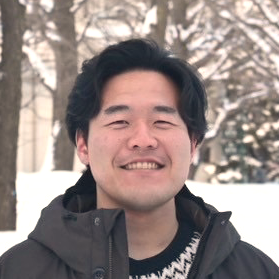
\includegraphics[width=31mm]{face.png}
\end{textblock}

\begin{rSection}{研究分野 (Research Interest)}
ヒューマンコンピュータインタラクション（HCI）, インタラクションデザイン, \\アクセシビリティ, センシング, ジェスチャ認識, UI/UX
\end{rSection}

%%%%%%%%%%%%	EDUCATION SECTION
\begin{rSection}{学歴 (Education)}
	
	\textbf{北海道大学大学院情報科学院 情報科学専攻} \hfill \textit{2024年4月 --- 現在（2027年3月卒業予定）} \\ 
	博士（情報科学）{\scriptsize \hfill 指導教員：坂本 大介}
    
    \textbf{北海道大学大学院情報科学院 情報科学専攻} \hfill \textit{2022年4月 --- 2024年3月} \\ 
	修士（情報科学） {\scriptsize \hfill 指導教員：坂本 大介}

    \textbf{北海道大学 工学部 情報理工学科} \hfill \textit{2020年4月 --- 2022年3月} \\ 
	学士（工学）{\scriptsize \hfill 指導教員：小野 哲雄, 坂本 大介}

    \textbf{岐阜工業高等専門学校 電気情報工学科} \hfill \textit{2015年4月 --- 2020年3月} \\ 
	準学士（工学）{\scriptsize \hfill 指導教員：出口 利憲}
    	
\end{rSection}
\begin{rSection}{職歴 (Work Experience)}
    \textbf{シンガポールマネジメント大学 Visiting Research Student} \hfill \textit{2026年3月 --- 2026年10月} \\ 
    {\scriptsize \hfill 担当：原 航太郎}
    
    \textbf{ラインヤフー株式会社 リサーチインターン} \hfill \textit{2023年3月 --- 2024年6月} \\ 
    {\scriptsize \hfill 担当：池松 香}
\end{rSection}

%%%%%%%%%%%%	WORK EXPERIENCE SECTION
\begin{rSection}{研究業績 (Papers)}
    
	\begin{rSubsection}{査読付き国際会議 (Peer-reviewed International Conferences)}{}{}{}
        \item \underline{\textbf{Kan Kusakabe}}, Yuki Abe, Karthick Anandan, Daisuke Sakamoto, Kotaro Hara. Enhancing Object Retrieval via Phase-Aware 3D Spatial Guidance for Blind and Low-Vision Users. The 2026 ACM International Joint Conference on Pervasive and Ubiquitous Computing (UbiComp 2026), Poster, Shanghai, October 2026. (\textbf{Best Poster Award Runner-up}). [DOI: TBD]
        \item Yuki Abe*, \underline{\textbf{Kan Kusakabe*}}, Myungguen Choi*, Daisuke Sakamoto, Tetsuo Ono. *Joint first authors. Understanding Usability of VR Pointing Methods with a Handheld-style HMD for Onsite Exhibitions. ACM CHI Conference on Human Factors in Computing Systems (CHI 2025), ACM, 2025. (\textbf{Honorable Mentions: top 5 \% of submitted papers}). [\href{https://doi.org/10.1145/3706598.3713874}{doi}]
    \end{rSubsection}

    \begin{rSubsection}{査読付き論文誌 (Peer-reviewed Journals)}{}{}{}
		\item \underline{\textbf{日下部 完}}, 池松 香, 坂本 大介, 小野 哲雄. BodSockets：スマホソケット型インタフェースを用いたスマートフォンの背面領域を活用した操作手法の提案. 情報処理学会論文誌，情報処理学会, Vol. 66 (12). [\href{https://doi.org/10.20729/0002006344}{doi}]
        
		\item \underline{\textbf{日下部 完}}, 坂本 大介, 小野 哲雄. RingSense：スマートフォン背面のジェスチャ入力を実現するスマホリング型インタフェースの設計と実装. 情報処理学会論文誌，情報処理学会, Vol. 66 (2). [\href{https://doi.org/10.20729/0002000028}{doi}]
    \end{rSubsection}

    \begin{rSubsection}{査読付き国内会議 (Peer-reviewed Domestic Conferences)}{}{}{}
		\item 豊田 真吾, \underline{\textbf{日下部 完}}, 坂本 大介. KanaShark: SHARK2に基づく日本語ジェスチャ入力手法の検討. 第33回インタラクティブシステムとソフトウェアに関するワークショップ（WISS 2025），日本ソフトウェア科学会，2025年12月. (スポンサー賞). [\href{www.wiss.org/WISS2025/downloads/proceedings.pdf}{pdf}]
        
		\item 小林 広夢, 鈴木 湧登, \underline{\textbf{日下部 完}}, 坂本 大介. 座位での物理的な制約の緩和を目指した知覚されない閾値に基づいたリダイレクション手法の提案と評価. 第33回インタラクティブシステムとソフトウェアに関するワークショップ（WISS 2025），日本ソフトウェア科学会，2025年12月. [\href{www.wiss.org/WISS2025/downloads/proceedings.pdf}{pdf}] 
        
		\item \underline{\textbf{日下部 完}}, 坂本 大介, 小野 哲雄. スマートフォン背面のジェスチャ入力を実現するスマホリング型デバイスの設計と実装. 第30回インタラクティブシステムとソフトウェアに関するワークショップ（WISS 2022），日本ソフトウェア科学会, pp.8-14，2022年12月. (ロング発表, 採択率：12.5\%). [\href{www.wiss.org/WISS2022Proceedings/data/02.pdf}{pdf}]
	\end{rSubsection}
	\begin{rSubsection}{その他の発表・デモ・ポスター (Other Publications)}{}{}{}
        \item \underline{\textbf{日下部 完}}, 阿部 優樹, Jaylee Soh, Karthick Anandan, 坂本 大介, 原 航太郎. PhaseNav: 段階的な空間誘導による視覚障がい者の物体取得支援. 第34回インタラクティブシステムとソフトウェアに関するワークショップ（WISS 2026），日本ソフトウェア科学会，2026年12月. (デモ発表). [\href{https://www.wiss.org/WISS2026/demo.html}{url}]
        \item \underline{\textbf{日下部 完}}, 阿部 優樹, 坂本 大介. BeMyARm：カメラエイミングを補助する視覚障がい者のための物体探索システムの提案. 第33回インタラクティブシステムとソフトウェアに関するワークショップ（WISS 2025），日本ソフトウェア科学会，2025年12月. (デモポスター発表).

		\item \underline{\textbf{日下部 完*}}, 阿部 優樹*, 坂本 大介, 小野 哲雄. *共同第一著者. Game-2-X: 種類が異なるゲームプレイ間を繋ぐシステムの提案. 第31回インタラクティブシステムとソフトウェアに関するワークショップ（WISS 2023），日本ソフトウェア科学会, 2023年12月. (デモンストレーション発表). [\href{www.wiss.org/WISS2023Proceedings/data/1-A03.pdf}{pdf}]
        
		\item \underline{\textbf{日下部 完}}, 崔 明根, 坂本 大介, 小野 哲雄. 無段階調整インタフェースのためのハンドジェスチャによる操作手法の探索的研究. 情報処理学会 研究報告ヒューマンコンピュータインタラクション（HCI）, 2022-HCI-197(25), 1-8, 2022年3月. [\href{ipsj.ixsq.nii.ac.jp/records/217445}{web}]
	\end{rSubsection}

    \begin{rSubsection}{招待講演・トップコンファレンスセッション (Invited Talks)}{}{}{}
        \item 阿部 優樹*，\underline{\textbf{日下部 完*}}，崔 明根*，坂本 大介，小野 哲雄. *共同第一著者. 展示空間における手持ち型ヘッドマウントディスプレイのVRポインティング手法の検討. 第33回インタラクティブシステムとソフトウェアに関するワークショップ（WISS 2025），日本ソフトウェア科学会，2025年12月. (国際学会招待発表).
        
        \item 阿部 優樹*，\underline{\textbf{日下部 完*}}，崔 明根*，坂本 大介，小野 哲雄. *共同第一著者. 展示空間における手で掴むヘッドセットのVRポインティング手法の検討. 第24回情報科学技術フォーラム（FIT2025），一般社団法人電子情報通信学会，2025年9月. (トップコンファレンスセッション).
	\end{rSubsection}

\end{rSection}

%%%%%%%%%%%%	AWARDS SECTION
\begin{rSection}{受賞 (Awards)}
	\item \textbf{Best Poster Award Runner-up}, UbiComp 2026, 2026年10月. Enhancing Object Retrieval via Phase-Aware 3D Spatial Guidance for Blind and Low-Vision Users. [\href{https://www.ubicomp.org/ubicomp-iswc-2026/awards-all/}{url}]
	\item \textbf{スポンサー賞（企業賞：Dentsu Lab Tokyo賞）}, WISS 2025, 2025年12月. KanaShark: SHARK2に基づく日本語ジェスチャ入力手法の検討. [\href{https://www.wiss.org/WISS2025/award.html}{url}]
	\item \textbf{Honorable Mention Award（投稿論文の上位5\%）}, ACM CHI 2025, 2025年4月. Understanding Usability of VR Pointing Methods with a Handheld-style HMD for Onsite Exhibitions. [\href{https://programs.sigchi.org/chi/2025/awards/honorable-mentions}{url}]
\end{rSection}
\begin{rSection}{学会活動・貢献 (Service)}{}{}{}
    - ACM CHI 2027 査読 (Paper Track)

    - ACM CHI 2026 査読 (Paper Track)
\end{rSection}

\begin{rSection}{フェローシップ・助成金 (Fellow)}
    1. 北海道大学 EXEX博士後期課程フェローシップ. 2024年--2027年. 400,000（¥/year）および生活費等支給.
    
    2. 北大テックガレージ (HOKUDAI TECH GARAGE) プロジェクト. 2ヶ月間 (2022年3月--4月), 1プロジェクトにつき300,000¥.
\end{rSection}


%%%%%%%%%%%%	TECHNICAL STRENGTHS SECTION
\needspace{9\baselineskip} % 見出しだけがページ末に残らないようにする
\begin{rSection}{技術・スキル (Technical Strengths)}
    - \textbf{分野}: ラピッドプロトタイピング, 3Dプリント, モバイルアプリ開発, 機械学習 (ML)

    - \textbf{プログラミング言語}:
    Python, C, C\#, JavaScript, PHP, Swift, Objective-C, Kotlin, Java, Arduino, Processing, Dart, \LaTeX

    - \textbf{フレームワーク・ライブラリ}:
    Tensorflow, Pytorch, Next.js, Flutter, React, Unity
    
    - \textbf{プラットフォーム・開発環境}:
    Android, iOS, Web (フロントエンド, バックエンド, データベース), Mac, Arduino Platform, Raspberry Pi

    - \textbf{デザイン}:
    Adobe (Illustrator, Photoshop, Premiere Pro, After Effects, Audition, Figma), Fusion 360
\end{rSection}
\end{document}